Currently, every drawers are connected with the main controller via wires. However, this wires reduce the user friendliness, if an user pull out the drawer completely. For the purpose of fast and cost effective prototype implementation we restrict ourself to implement such a sophistical system. The idea of making each drawer independent of wire is placing connection pins bottom of the drawers and also the out going wire to the controller 
should be placed with small plate in the main structure of the shelf, so that the when the drawer is closed each of the drawer get a connection between the pins and plate and make bridge between the drawers and controller.
There figure \ref{fig:connector} shows the idea of implementing such a drawer with a very minimalistic complexity.
%
\begin{figure}
	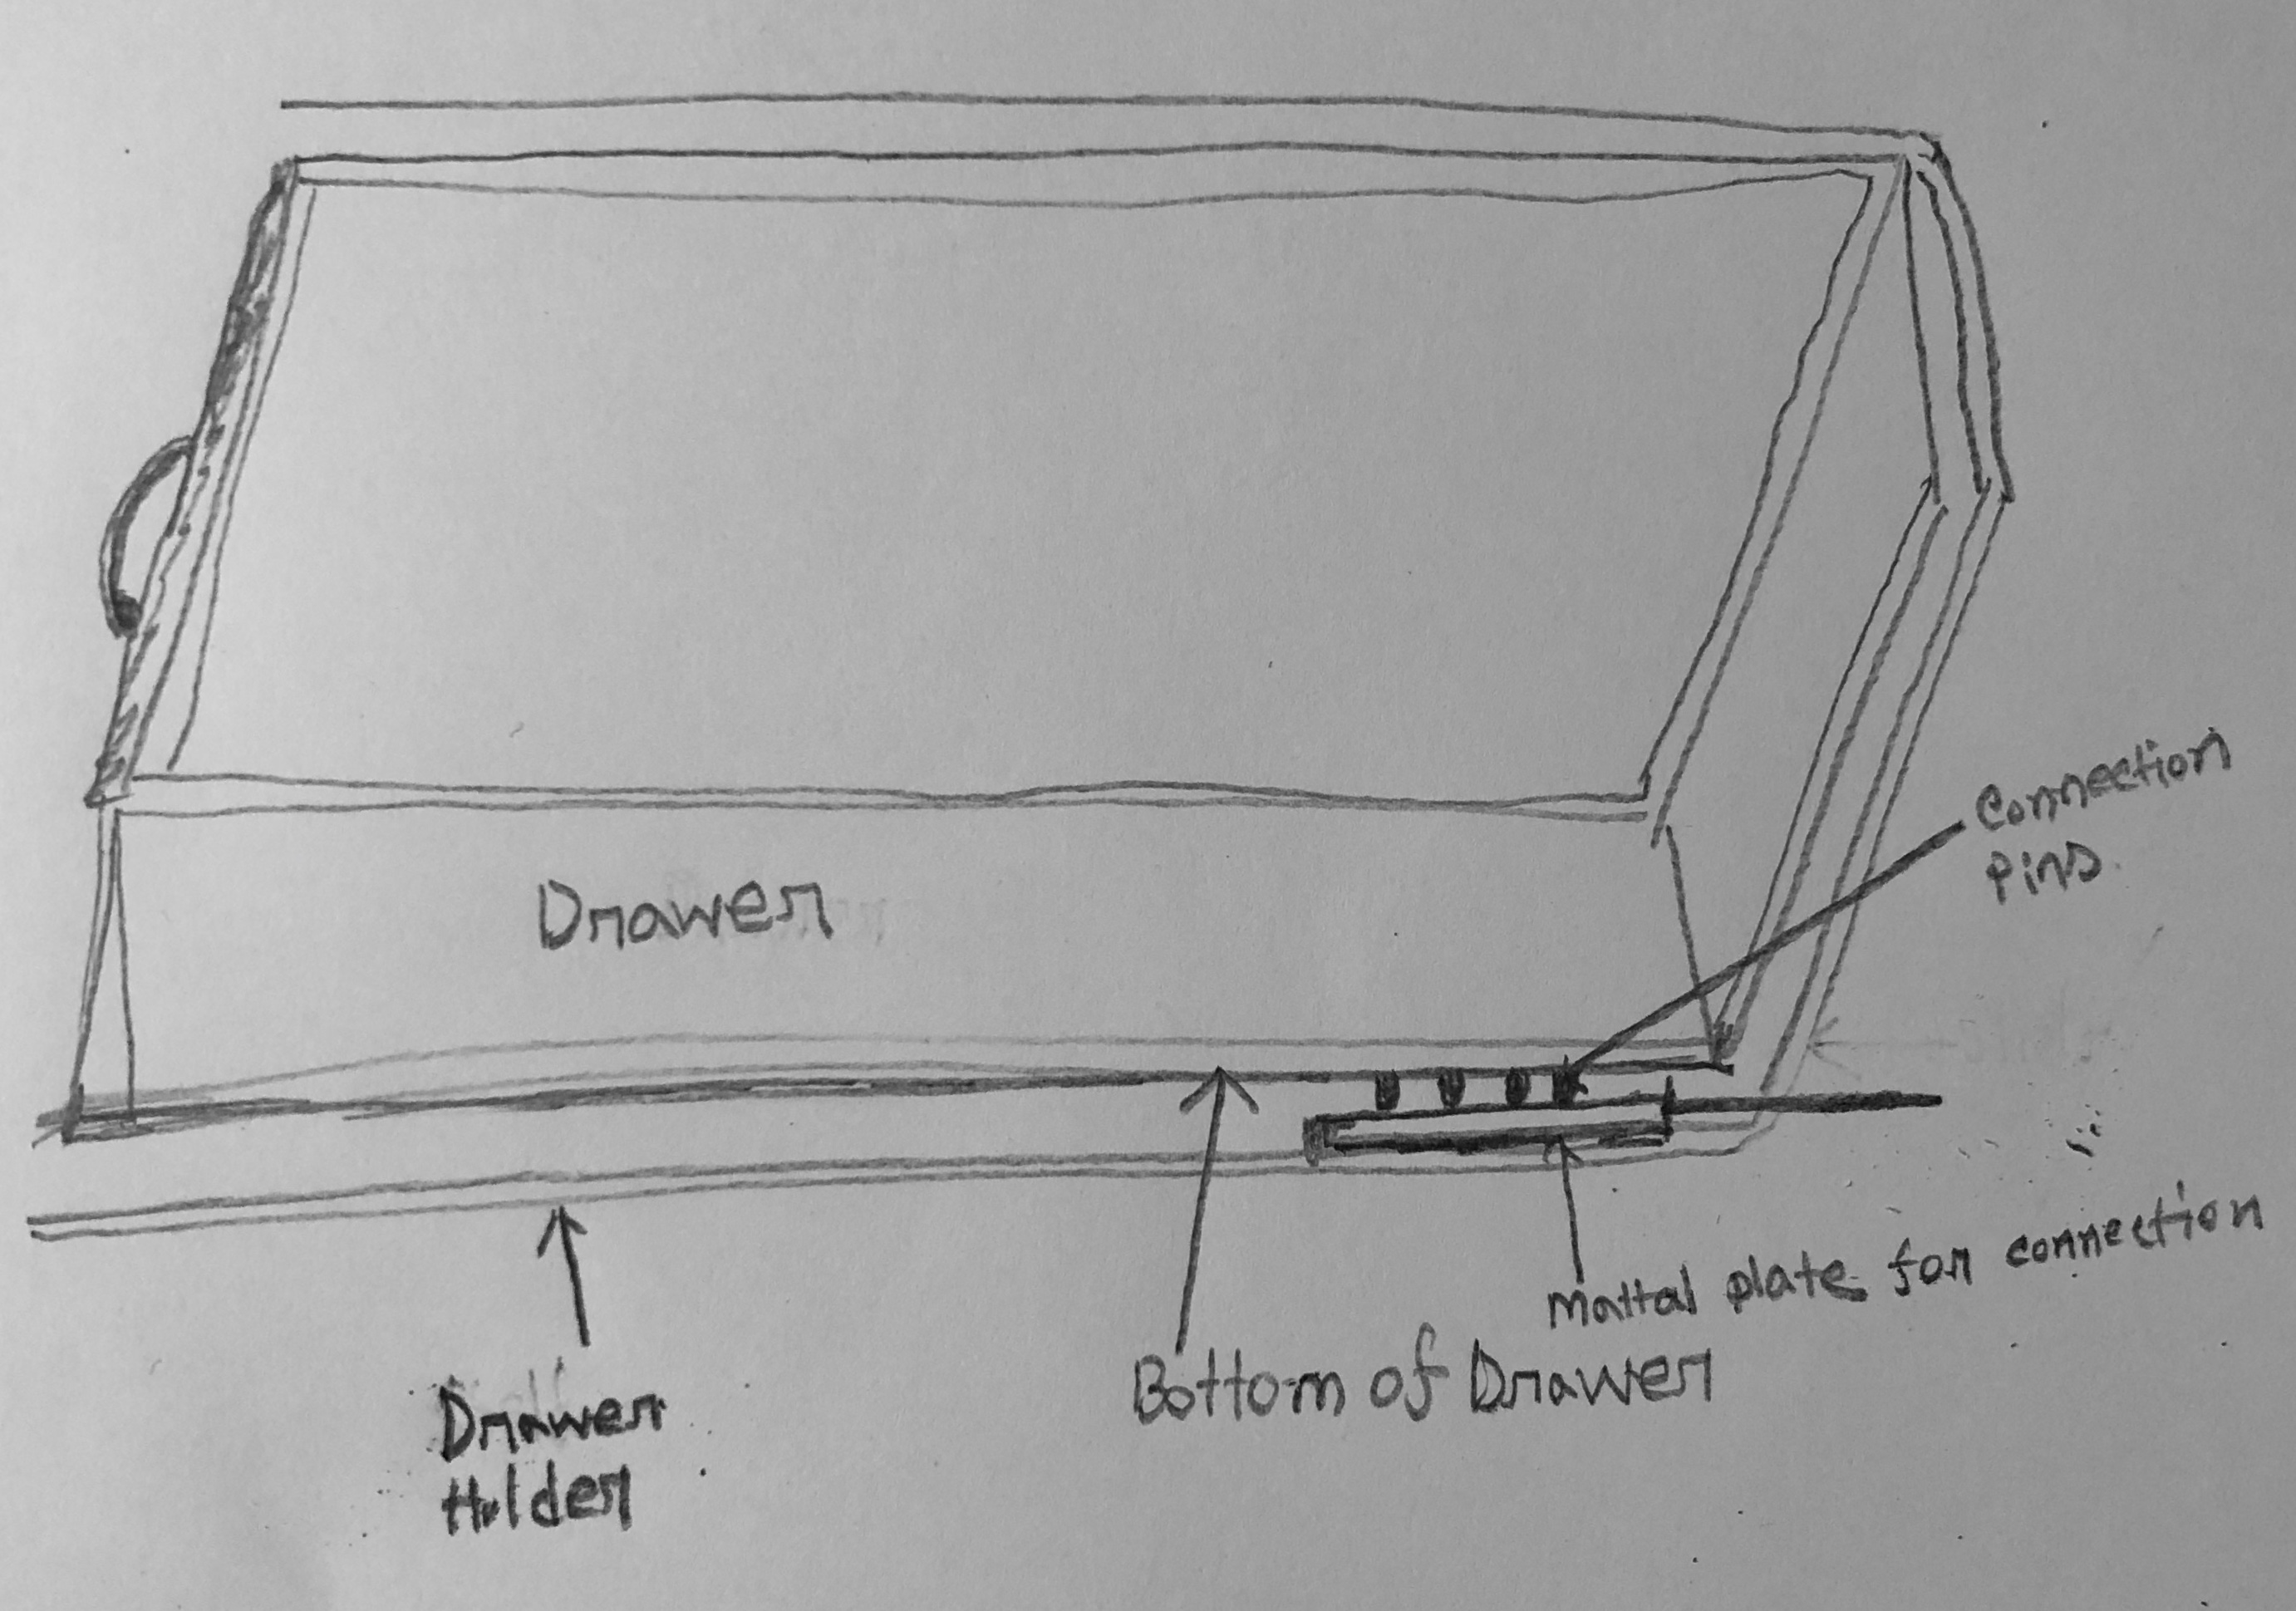
\includegraphics[width=1\columnwidth]{figures/connector}
	\caption{Sketch of connector for removing dependency on connecting wires}~\label{fig:connector}
\end{figure}
%
\\
\\